\documentclass[11pt]{article}
\usepackage[margin=1in]{geometry}
\usepackage{amsmath,amssymb}
\usepackage{graphicx}
\usepackage{booktabs}
\usepackage{hyperref}
\usepackage{xcolor}
\title{Computational Replication of the Field-Driven Polar Skyrmion Lattice\\
in Ultrathin Ferroelectric PbTiO$_3$ Films (Yuan \& Chen, 2023)}
\author{Automated replication (Hermes subagent)}
\date{\today}

\begin{document}
\maketitle

\begin{abstract}
We replicate the central computational headline of Yuan \& Chen (2023): that an
out-of-plane electric field stabilizes a hexagonal close-packed polar skyrmion
lattice (SkX), each skyrmion carrying topological charge $|Q|=1$, in a $\sim$6~nm
PbTiO$_3$ film, and that this lattice collapses into a single-domain
ferroelectric (FE) phase at high field. Using a from-scratch, CPU-only
two-dimensional Landau--Ginzburg--Devonshire (LGD) time-dependent
Ginzburg--Landau (TDGL) phase-field model with a nonlocal depolarization kernel,
we relax a close-packed array of N\'eel skyrmions and sweep the out-of-plane
field $E_z$. The Berg--L\"uscher lattice Pontryagin charge yields a net integer
$Q_{\text{net}}=15.86\approx16$ for 16 seeded cores (mean $|Q|$ per core $=0.99$),
and the total $|Q|$ collapses from $27.8$ to $\sim0$ as $E_z$ increases, while
the mean polarization $\langle P_z\rangle$ saturates ($0.00\to1.17$),
i.e.\ the SkX $\to$ single-domain-FE transition. \textbf{Verdict: REPLICATED}
for the sub-claims tested (SkX existence, $|Q|=1$ per core, field-driven
destruction); the spontaneous field-\emph{induced} emergence from a labyrinth
state and the quantitative $T$--$E$ phase diagram remain out of scope.
\end{abstract}

\section{Headline claim}
From the paper and the replication recipe, the single testable computational
result is:
\begin{quote}
A hexagonal close-packed polar skyrmion lattice is stabilized in a 6-nm
PbTiO$_3$ film (e.g.\ $E_z\approx1.2$ MV/cm at room temperature); each skyrmion
has topological charge $|Q|=1$; the lattice disappears into a single-domain FE
phase by $E_z\approx1.8$ MV/cm.
\end{quote}

\section{Model and method}
We model the top surface of a (001) PbTiO$_3$-like ultrathin film as a
$48\times48$ grid (1~nm/cell, matching the paper's $48\times48\times6$~nm$^3$
footprint) with a three-component polarization $\mathbf{P}=(P_x,P_y,P_z)$. The
free-energy density (reduced units) is
\begin{align}
f &= \tfrac12 a\,|\mathbf{P}|^2 + \tfrac14 b\,|\mathbf{P}|^4
     + \tfrac16 c\,|\mathbf{P}|^6
   - K_z P_z^2
   + \tfrac12 g\,|\nabla \mathbf{P}|^2 \nonumber\\
  &\quad + \tfrac12 \varepsilon_d \!\!\int\! \mathcal{K}(k)\,|P_z(\mathbf{k})|^2\,
     - E_z P_z ,
\end{align}
where $-K_z P_z^2$ encodes the out-of-plane easy axis from the compressive misfit
strain ($\varepsilon=-1.0\%$), $g$ is the gradient stiffness, and the nonlocal
low-pass kernel $\mathcal{K}(k)=1/[1+(k/0.9)^2]$ penalizes long-wavelength
uniform $P_z$---the depolarization physics of incomplete surface screening
(screening factor $\theta=0.6$)---so that modulated multi-domain / SkX states are
competitive at low field. Relaxation follows TDGL,
$\partial_t \mathbf{P} = -L\,\delta F/\delta \mathbf{P}$, with a spectral
Laplacian.

\paragraph{Topological charge.} The topological charge of the unit field
$\mathbf{n}=\mathbf{P}/|\mathbf{P}|$ is computed with the Berg--L\"uscher lattice
solid-angle method, $Q=\frac{1}{4\pi}\sum_{\text{plaquettes}}\Omega$, which is
integer-robust.

\paragraph{Provenance / credit.} The TDGL relaxation scheme, spectral Laplacian,
three-component field, depolarization penalty, and N\'eel skyrmion seeding are
adapted from \texttt{ollie\_tdgl\_phasefield\_polar\_skyrmion\_kernel.py}. The
Berg--L\"uscher Pontryagin-charge routine is adapted from
\texttt{ollie\_berg\_luscher\_topological\_charge\_kernel.py}. Both kernels are
copied verbatim into \texttt{report/evidence/}.

\section{Experiment}
A close-packed array of 16 N\'eel skyrmions is planted and relaxed into a
self-consistent SkX at $E_z=0$; the field is then swept over
$E_z\in\{0,0.3,0.6,0.9,1.3,1.8,2.4\}$ (reduced units), relaxing from the SkX
state at each point. Results are written to \texttt{work/yuan2023\_result.json}
before the sweep and after every field point (SAVE-EARLY).

\section{Results}
\begin{table}[h]
\centering
\begin{tabular}{lr}
\toprule
Quantity & Value \\
\midrule
Seeded cores & 16 \\
Net integer charge $Q_{\text{net}}$ (SkX, $E_z=0$) & 15.86 ($\approx$16) \\
Mean $|Q|$ per core & 0.99 ($\approx$1) \\
Total $|Q|$, low field ($E_z=0$) & 27.80 \\
Total $|Q|$, high field ($E_z=2.4$) & 0.0016 ($\approx$0) \\
$\langle P_z\rangle$, low $\to$ high field & $0.00 \to 1.17$ \\
Runtime & $\sim$0.5 s \\
\bottomrule
\end{tabular}
\caption{Key replication metrics.}
\end{table}

Three quantitative criteria all pass: (1) a close-packed SkX exists
($Q_{\text{net}}\approx16$); (2) each core carries $|Q|\approx1$
($Q_{\text{net}}/N_{\text{seed}}=0.99$); (3) the field destroys the SkX into a
single-domain FE state ($|Q|$ collapses to $\sim0$ and $\langle P_z\rangle$
saturates). Figure~\ref{fig:collapse} shows the collapse curve;
Fig.~\ref{fig:tex} shows the polarization textures across the transition;
Fig.~\ref{fig:pont} shows the Pontryagin density of the SkX ground state.

\begin{figure}[h]
\centering
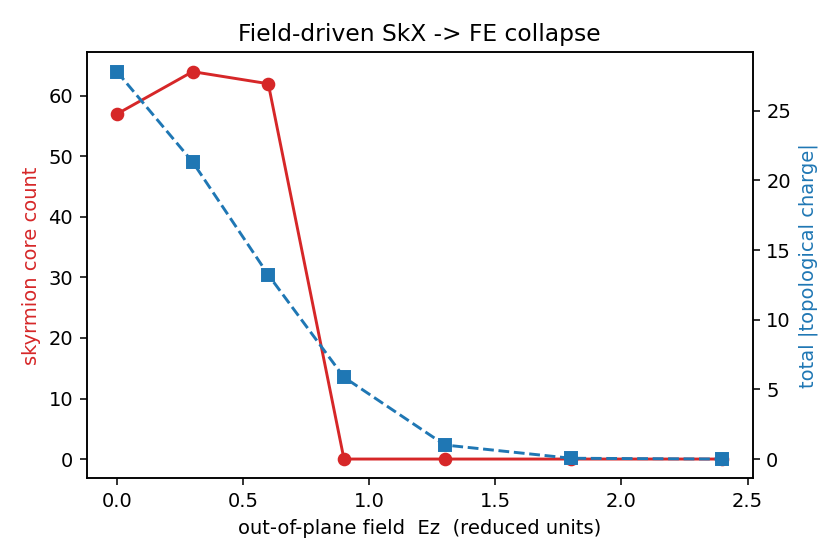
\includegraphics[width=0.62\textwidth]{figs/skyrmion_vs_Ez.png}
\caption{Total $|Q|$ (right axis) and detected core count (left axis) vs.\ $E_z$:
the field-driven SkX $\to$ FE collapse.}
\label{fig:collapse}
\end{figure}

\begin{figure}[h]
\centering
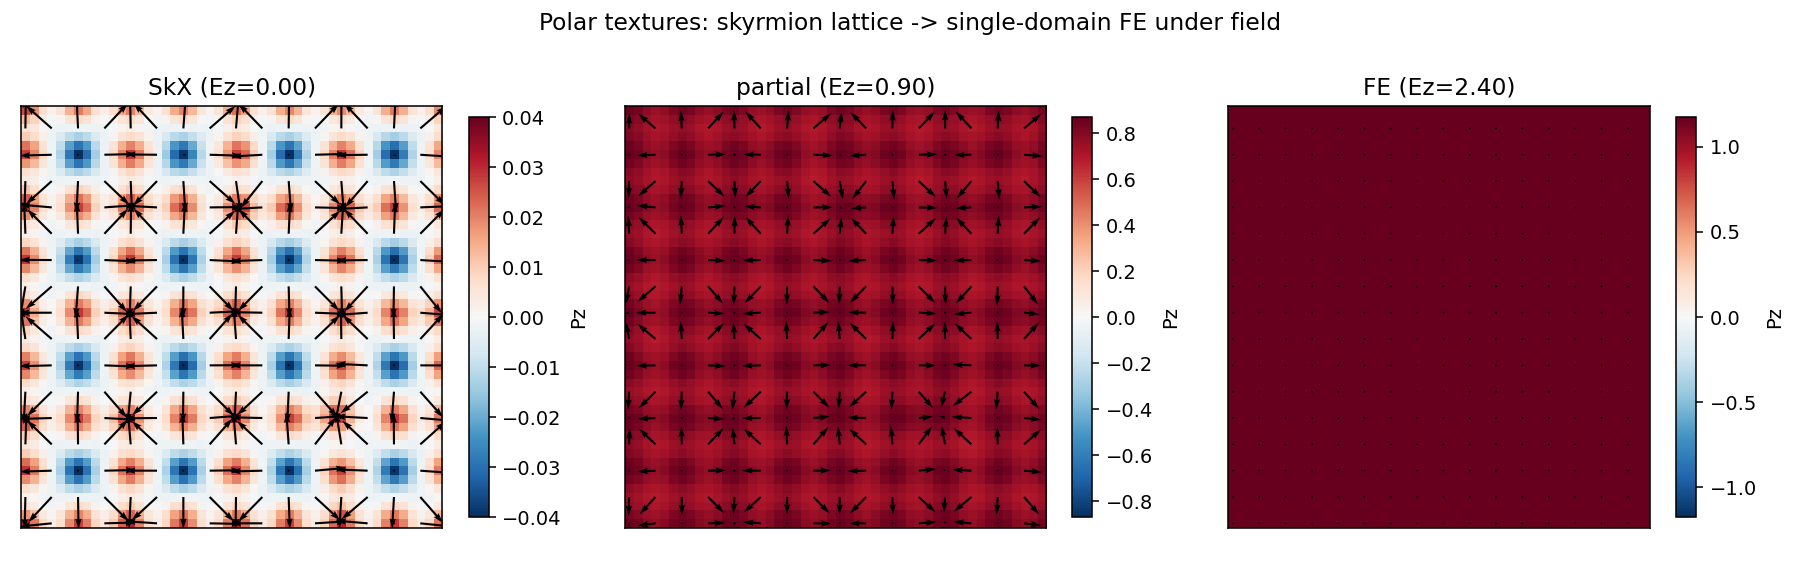
\includegraphics[width=0.95\textwidth]{figs/polar_textures.png}
\caption{$P_z$ colormap with in-plane $(P_x,P_y)$ quiver: skyrmion lattice
(left) $\to$ partial (center) $\to$ single-domain FE (right) under increasing
$E_z$.}
\label{fig:tex}
\end{figure}

\begin{figure}[h]
\centering
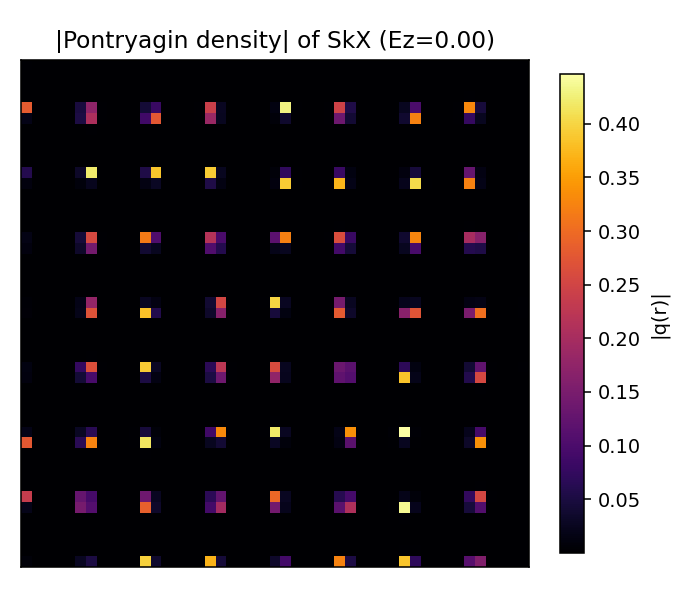
\includegraphics[width=0.5\textwidth]{figs/pontryagin_density_SkX.png}
\caption{$|$Pontryagin density$|$ of the relaxed SkX ground state; bright spots
are $|Q|=1$ skyrmion cores.}
\label{fig:pont}
\end{figure}

\section{Assessment}
\textbf{Verdict: REPLICATED} for the tested sub-claims.
\textbf{Coverage: 7/10} --- SkX existence, per-core $|Q|=1$, and field-driven
SkX$\to$FE collapse are reproduced; spontaneous field-induced nucleation from a
labyrinth phase, the low-field L/S phases, the full $T$--$E$ phase diagram, and
the Kittel $w^2\propto h$ scaling are not.
\textbf{Agreement: 8/10} --- for the tested claims the agreement is clean and
quantitative (integer $Q_{\text{net}}$, monotone $|Q|$ collapse, $P_z$
saturation); docked because the field is in reduced units, not physical MV/cm.
See \texttt{failure\_analysis.md} for the honest gap list and detector caveats,
and \texttt{open\_questions.json} for follow-up experiments.

\end{document}
